%%%%%%%%%%%%%%%%%%%%%%%%%%%%%%%%%%%%%%%%%%%%%%%%%%%%%%%%%%%%%%%%%%%%%%
% Overleaf (WriteLaTeX) Example: Molecular Chemistry Presentation
%
% Source: http://www.overleaf.com
%
% In these slides we show how Overleaf can be used with standard 
% chemistry packages to easily create professional presentations.
% 
% Feel free to distribute this example, but please keep the referral
% to overleaf.com
% 
%%%%%%%%%%%%%%%%%%%%%%%%%%%%%%%%%%%%%%%%%%%%%%%%%%%%%%%%%%%%%%%%%%%%%%

\documentclass{beamer}

\mode<presentation>
{
  \usetheme{Madrid}       % or try default, Darmstadt, Warsaw, ...
  \usecolortheme{default} % or try albatross, beaver, crane, ...
  \usefonttheme{default}    % or try default, structurebold, ...
  \setbeamertemplate{navigation symbols}{}
  \setbeamertemplate{caption}[numbered]
} 

\usepackage[english]{babel}
\usepackage[utf8x]{inputenc}
\usepackage{chemfig}
\usepackage[version=3]{mhchem}

\usepackage{siunitx}
  \sisetup{separate-uncertainty = true}
\usepackage{physics}
\usepackage[font=small,labelfont=bf]{caption}
\usepackage{subcaption}
\usepackage[en-GB]{datetime2}
\usepackage{feynmp}
\DeclareGraphicsRule{*}{mps}{*}{}

\usepackage{scalerel}
\newcommand{\mylbrace}[2]{\vspace{#2pt}\hspace{6pt}\scaleleftright[\dimexpr5pt+#1\dimexpr0.06pt]{\lbrace}{\rule[\dimexpr2pt-#1\dimexpr0.5pt]{-4pt}{#1pt}}{.}}
\newcommand{\myrbrace}[2]{\vspace{#2pt}\scaleleftright[\dimexpr5pt+#1\dimexpr0.06pt]{.}{\rule[\dimexpr2pt-#1\dimexpr0.5pt]{-4pt}{#1pt}}{\rbrace}\hspace{6pt}}

% Here's where the presentation starts, with the info for the title slide
\title[$B^\pm\to(K^+K^-\pi^+\pi^-)_DK^\pm$]{Measuring \texorpdfstring{$\gamma$}{gamma} in \texorpdfstring{$B^\pm\to(K^+K^-\pi^+\pi^-)_DK^\pm$}{B to K+K-pi+pi-} decays}
\author{Martin Tat}
\institute{Oxford LHCb}
\date{\today}

\begin{document}

\begin{frame}
  \titlepage
\end{frame}

% These three lines create an automatically generated table of contents.
\begin{frame}{Outline}
  \tableofcontents
\end{frame}

\section{Background}
\begin{frame}{Background}
  \begin{itemize}
    \item 4-year MPhys in Oxford
    \begin{itemize}
      \item Performance of monolithic CMOS sensors
      \item Prof Daniela Bortoletto
    \end{itemize}
    \item CERN Summer Student 2019
    \begin{itemize}
      \item Beam loss reduction in TT$20$ transfer line
      \item Dr Yann Dutheil, Dr Matthew Fraser
    \end{itemize}
    \item Oxford Summer Student 2018
    \begin{itemize}
      \item Study of PDF uncertainties in W-boson mass measurement
      \item Prof Chris Hays
    \end{itemize}
    \item RAL Summer Student 2018
    \begin{itemize}
      \item Bending magnets in accelerator simulations (Dr Chris Rogers)
    \end{itemize}
  \end{itemize}
\end{frame}

\section{\texorpdfstring{$\gamma$}{gamma} and the unitary triangle}
\begin{frame}{$\gamma$ and the unitary triangle}
  \begin{center}
    Unitarity of CKM matrix: $V_{ud}V^*_{ub} + V_{cd}V^*_{cb} + V_{td}V^*_{tb} = 0$ \\
    \vspace{0.4cm}
    Define $\gamma = \text{arg}\Big(-\frac{V_{ud}V^*_{ub}}{V_{cd}V^*_{cb}}\Big)$
  \end{center}
  \vspace{-0.2cm}
  \begin{figure}
    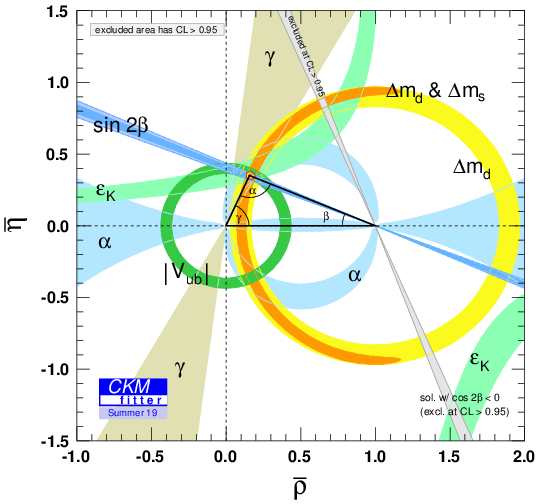
\includegraphics[scale = 0.3]{ckmfitter.png}
  \end{figure}
  \vspace{-0.4cm}
  \begin{center}
    CKMfitter Group (J. Charles et al.), Eur. Phys. J. C41, 1-131 (2005)
  \end{center}
\end{frame}

\begin{frame}{\texorpdfstring{$\text{b}\to\text{u}$}{b to u} and \texorpdfstring{$\text{b}\to\text{c}$}{b to c} interference}
  \begin{figure}[H]
    \centering
    \vspace{0.3cm}
    \begin{subfigure}{0.5\textwidth}
      \centering
      \begin{fmffile}{fgraph_BtoDK1}
        \setlength{\unitlength}{0.4cm}
        \begin{fmfgraph*}(6,6)
          \fmfstraight
          \fmfleft{i1,B,i2,t1,t2,t3,t9,t10}
          \fmfright{o1,D,o2,t4,t5,o3,K,o4}
          \fmflabel{$\bar{u}$}{i1}
          \fmflabel{$b$}{i2}
          \fmfv{l.d=20,l.a=180,l={$B^-$\mylbrace{30}{-8}}}{B}
          \fmflabel{$\bar{u}$}{o1}
          \fmflabel{$c$}{o2}
          \fmflabel{$\bar{u}$}{o3}
          \fmflabel{$s$}{o4}
          \fmfv{l.d=15,l.a=0,l={\myrbrace{30}{-12}}$D^0$}{D}
          \fmfv{l.d=15,l.a=0,l={\myrbrace{30}{11}}$K^-$}{K}
          \fmf{fermion}{o1,i1}
          \fmf{fermion,tension=1.5}{i2,v1}
          \fmf{fermion}{v1,o2}
          \fmf{phantom,tension=1.5}{t9,v2}
          \fmf{boson,label=$W$,label.side=left,tension=0}{v1,v2}
          \fmf{fermion}{v2,o4}
          \fmf{fermion}{o3,v2}
        \end{fmfgraph*}
      \end{fmffile}
      \vspace{0.5cm}
      \caption{$B^-\to D^0K^-$}
    \end{subfigure}%
    \begin{subfigure}{0.5\textwidth}
      \centering
      \begin{fmffile}{fgraph_BtoDK2}
        \setlength{\unitlength}{0.4cm}
        \begin{fmfgraph*}(6,6)
          \fmfstraight
          \fmfleft{i1,t1,t2,B,t9,t10,i2}
          \fmfright{o1,K,o2,t4,t5,o3,D,o4}
          \fmflabel{$\bar{u}$}{i1}
          \fmflabel{$b$}{i2}
          \fmfv{l.d=20,l.a=180,l={$B^-$\mylbrace{100}{-8}}}{B}
          \fmflabel{$\bar{u}$}{o1}
          \fmflabel{$s$}{o2}
          \fmflabel{$\bar{c}$}{o3}
          \fmflabel{$u$}{o4}
          \fmfv{l.d=15,l.a=0,l={\myrbrace{30}{13}}$\bar{D^0}$}{D}
          \fmfv{l.d=15,l.a=0,l={\myrbrace{30}{-13}}$K^-$}{K}
          \fmf{fermion}{o1,i1}
          \fmf{fermion,tension=1.5}{i2,v1}
          \fmf{fermion}{v1,o4}
          \fmf{phantom,tension=1.5}{t2,v2}
          \fmf{boson,label=$W$,label.side=left,tension=0}{v1,v2}
          \fmf{fermion}{v2,o2}
          \fmf{fermion}{o3,v2}
        \end{fmfgraph*}
      \end{fmffile}
      \vspace{0.5cm}
      \caption{$B^-\to\bar{D^0}K^-$}
    \end{subfigure}
  \end{figure}
  \vspace{0.4cm}
  \begin{center}
    Similar diagrams for $B^+\to DK^+$, with $\gamma\to -\gamma \implies$ \\
    \vspace{0.3cm}
    Inteference when $D^0$ and $\bar{D^0}$ decay into a common final state
  \end{center}
\end{frame}

\subsection{The ch}
\begin{frame}{The chemistry packages}

We focus on two \LaTeX{} chemistry packages:
\begin{block}{The \texttt{chemfig} package}
This package provides the command which draws molecules. Created by Christian Tellechea, a detailed user guide can be found here:\\[0.4cm]
\small{\url{www.tex.ac.uk/ctan/macros/generic/chemfig/chemfig_doc_en.pdf}}
\end{block}
\begin{block}{The \texttt{mhchem} package}
The \texttt{mhchem} package provides simple commands for typesetting chemical molecular formulae and equations. Created by Martin Hensel, a detailed user guide can be found here:\\[0.4cm]
\small{\url{http://mirror.ox.ac.uk/sites/ctan.org/macros/latex/contrib/mhchem/mhchem.pdf}}
\end{block}

\end{frame}

\section{Using chemistry packages with \LaTeX{}}

\subsection{Chemical equations with \texttt{mhchem}}

\begin{frame}[fragile]
\frametitle{Chemical equations with \texttt{mhchem}}

\begin{itemize}
\item The \texttt{mhchem} package lets you write chemical equations in \LaTeX{} with the minimum of effort. 
\item The example below shows how the standard representation of a reaction (on the left) is created from the simple code on the right:
\end{itemize}

\begin{center}
\ce{CO2 + C -> 2CO} is created with \verb|\ce{CO2 + C -> 2CO}|
\end{center}

\begin{itemize}
\item More complicated reactions are still easy to write:
\end{itemize}

\begin{center}
\ce{SO4^2- + Ba^2+ -> BaSO4 v}\\[0.1cm]
is created with\\[0.1cm]
\verb|\ce{SO4^2- + Ba^2+ -> BaSO4 v}|
\end{center}

\end{frame}

\section{Where to go next\dots{}}

\begin{frame}{Where to go next\dots{}}

\begin{itemize}
\item This short example was designed to introduce you to using Overleaf for scientific presentations.
\item This is made possible by the many great packages that have been developed for \LaTeX{}, including the two we focused on here (plus the \texttt{Beamer} package used for the overall presentation style). 
\item For more help on using \LaTeX{}, see the links on the Overleaf help page: \url{www.overleaf.com/help} or check out our free introductory course: \url{www.overleaf.com/blog/7}.
\end{itemize}

\begin{center}
Follow @overleaf on Twitter for all the latest news and updates.\\[0.3cm]
Happy \LaTeX ing!
\end{center}

\end{frame}

\end{document}
